\documentclass[a4paper]{article}

%% Language and font encodings
\usepackage[english]{babel}
\usepackage[T1]{fontenc}

%% Sets page size and margins
\usepackage[a4paper,top=3cm,bottom=2cm,left=3cm,right=3cm,marginparwidth=1.75cm]{geometry}

%% Useful packages
\usepackage{amsmath}
\usepackage{graphicx}
\usepackage[colorlinks=true, allcolors=blue]{hyperref}

\title{Neural Networks Exercise 4}
\author{Jens, Mellberg, 11806523\\
		Group partner: Lassi, Lehtonen 11805955}

\begin{document}
\maketitle


   \begin{figure}[h]
\caption{Tanh, Learning rate: 0.2}
\centering
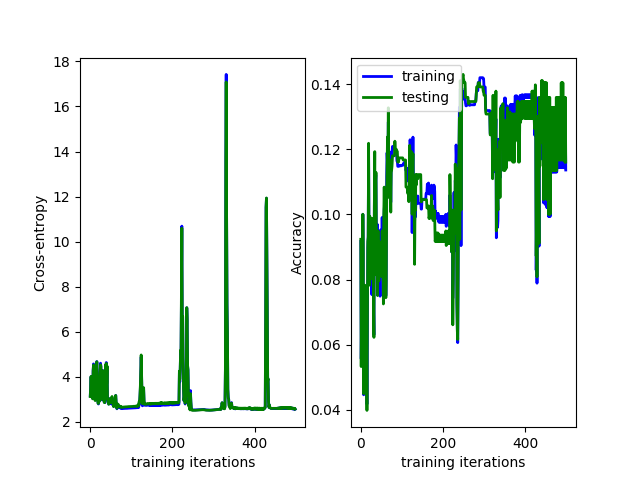
\includegraphics[width=15cm, height=12cm]{LR02.png}
\end{figure}

   \begin{figure}[h]
\caption{Tanh, Learning rate: 0.5}
\centering
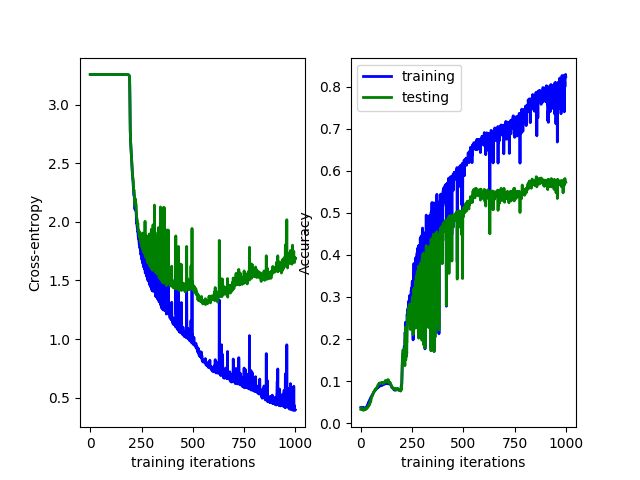
\includegraphics[width=15cm, height=12cm]{LR05.png}
\end{figure}

   \begin{figure}[h]
\caption{Tanh, Learning rate: 0.001}
\centering
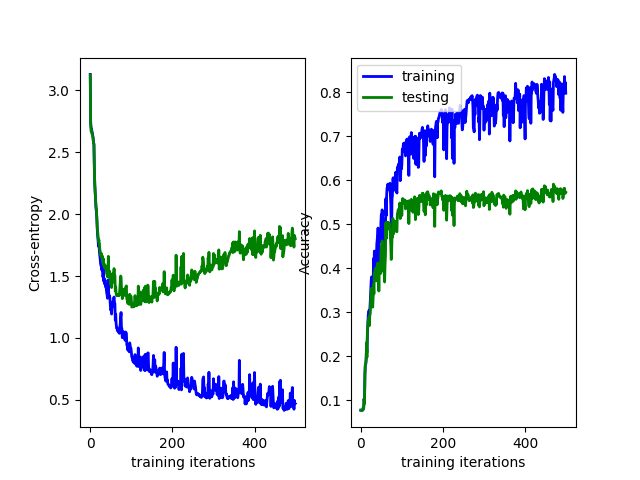
\includegraphics[width=15cm, height=12cm]{LR001.png}
\end{figure}

    

   \begin{figure}[h]
\caption{Relu, Learning rate: 0.001}
\centering
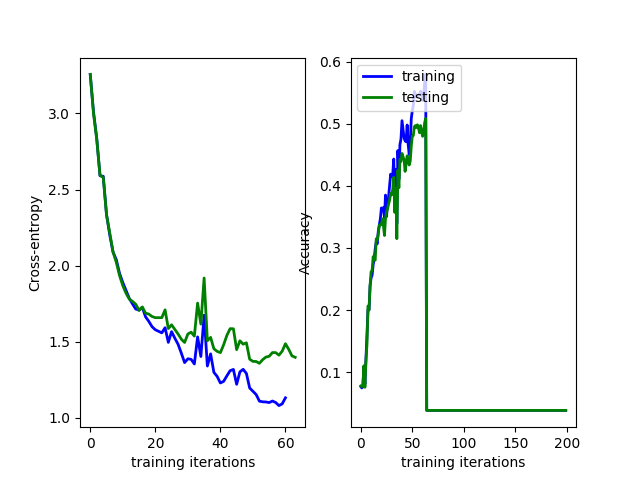
\includegraphics[width=15cm, height=12cm]{RELU001.png}
\end{figure}
    

\begin{figure}[h]
\caption{Relu, Learning rate: 0.00001}
\centering
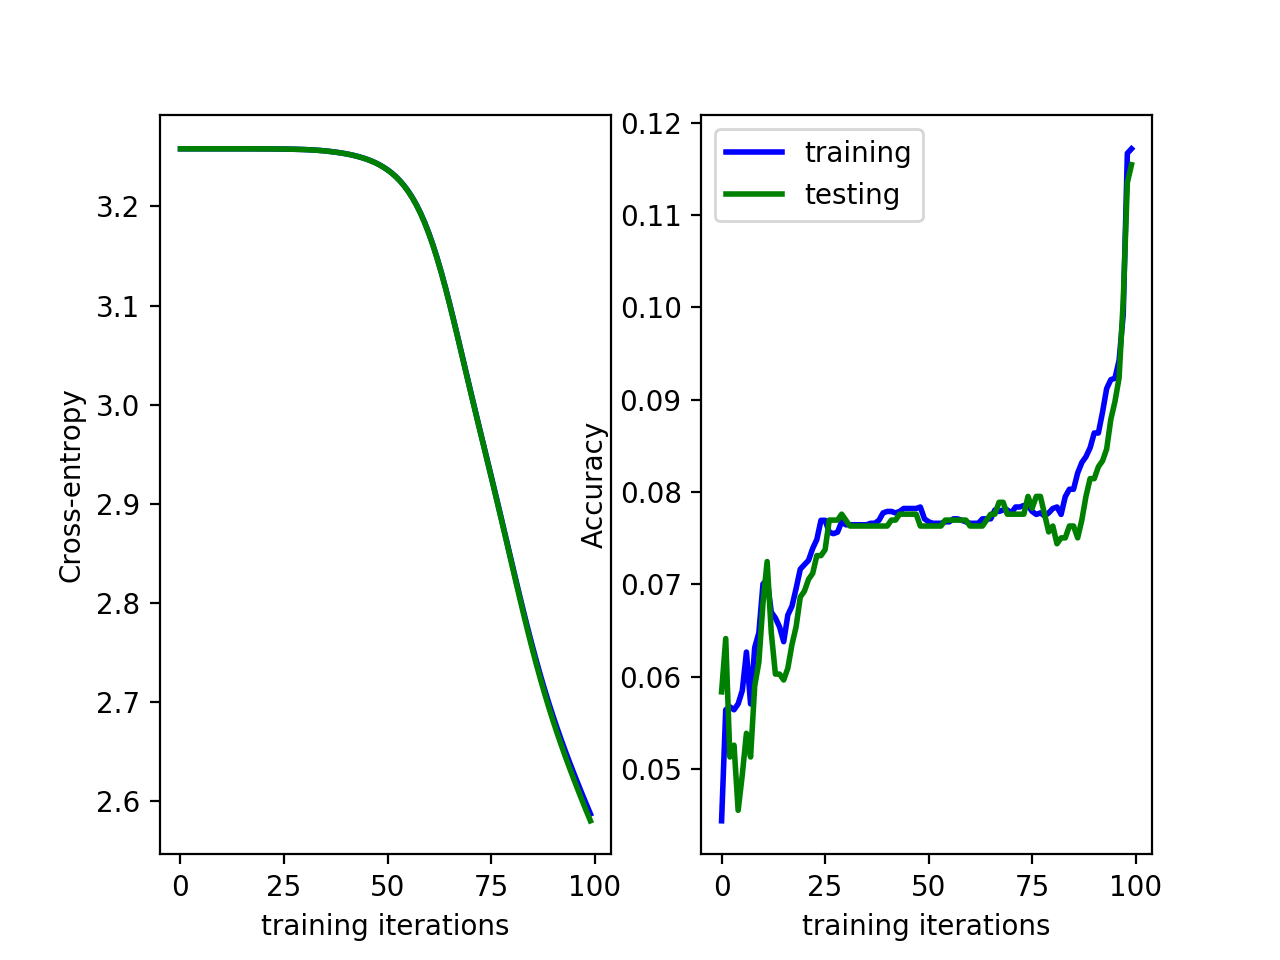
\includegraphics[width=15cm, height=12cm]{LR00001.png}
\end{figure}

\begin{figure}[h]
\caption{Relu, Learning rate: 0.00001}
\centering
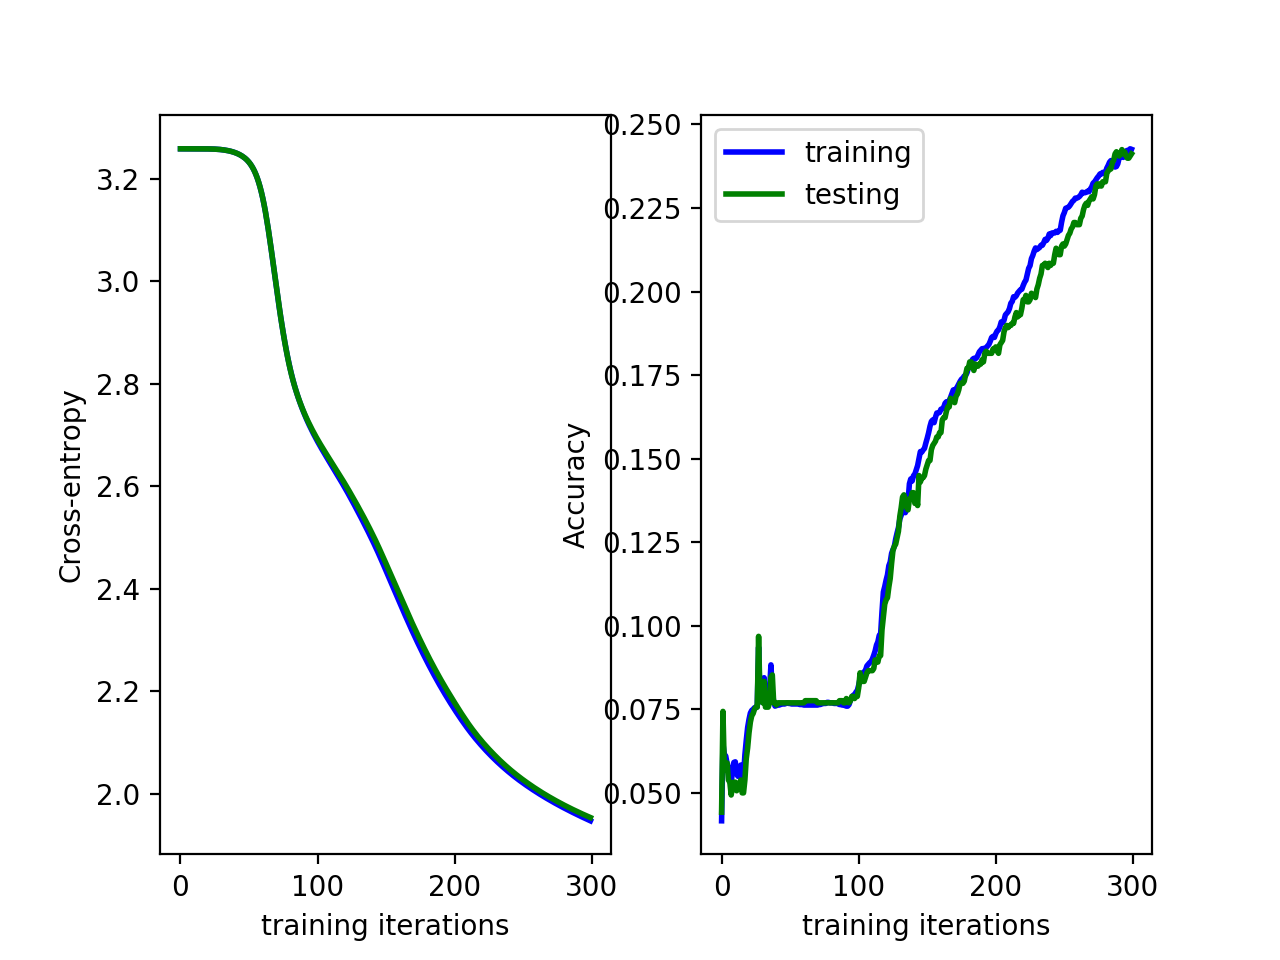
\includegraphics[width=15cm, height=12cm]{LR00001_2.png}
\end{figure}

\begin{figure}[h]
\caption{Relu, Learning rate: 0.00001}
\centering
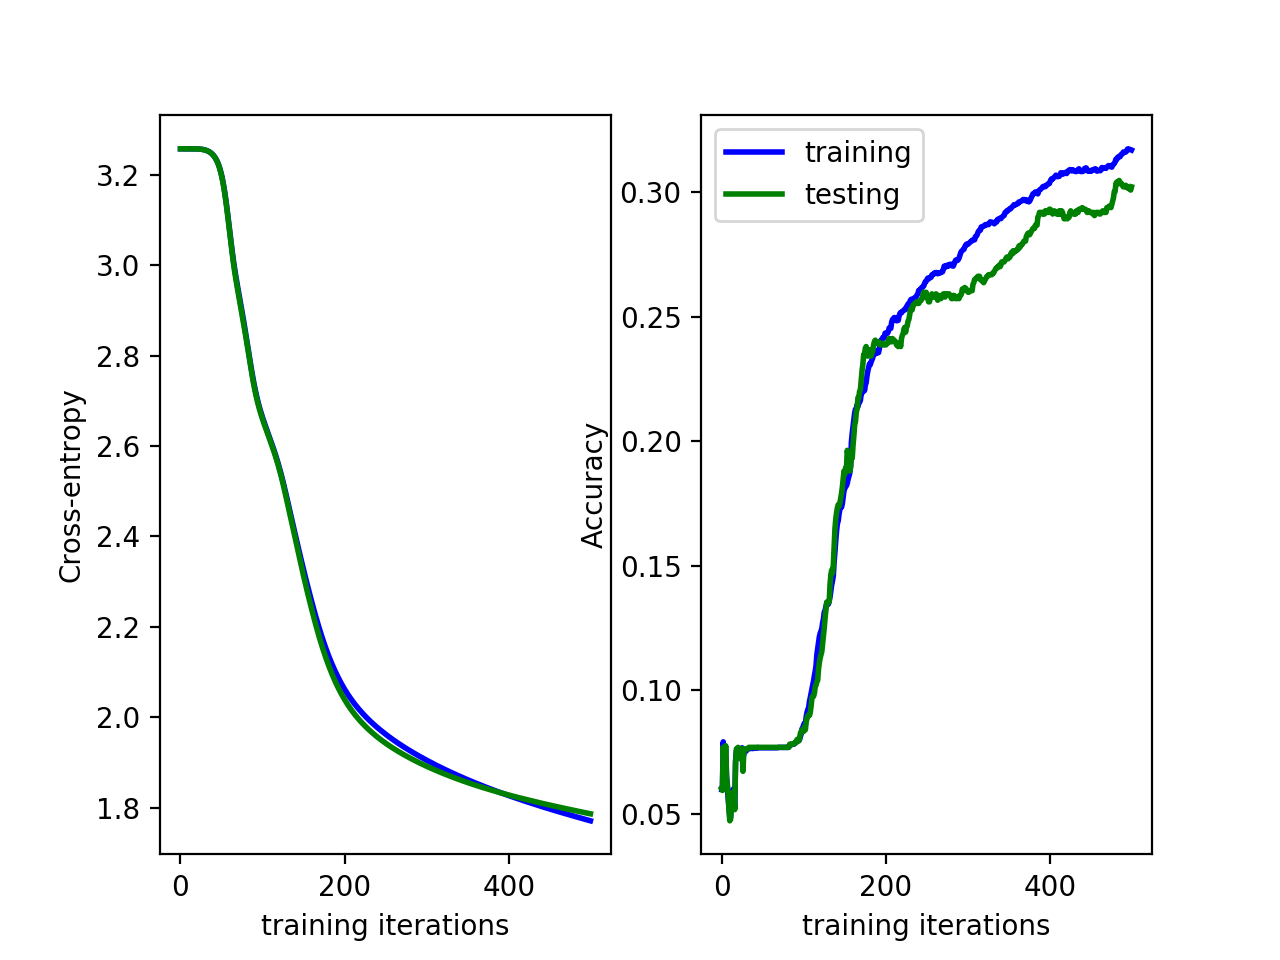
\includegraphics[width=15cm, height=12cm]{LR00001_3.png}
\end{figure}


As we see in the graphs, using the ReLu activation function with a too high learning rate will cause the network to get stuck with an accuracy of 0.038. We think this happens because too many neurons gets stuck with a constant output of 0 and never being able to recover.



\end{document}